% Appendices
% This should include detailed and technical documentation such as table of results, diagrams, program source code, etc, which are essential parts of the project but not directly a part of the main discussion in the report.  All contents of appendices should be exclusively, products of the student's own work.
% Other materials used during the project work (such as information from user manuals, interview notes, etc), which it is necessary to include, should if possible be summarized to only a few pages before entering into the appendix. Original copies of such material should be kept by the student and may be required to be produced as supporting evidence of their work.  Examples of key coding may be provided in an Appendix but generally it should be on the P drive with its associated software.
\section*{Appendices}
% https://stackoverflow.com/questions/72726606/latex-section-without-a-number-in-the-table-of-contents
\addcontentsline{toc}{section}{\protect\numberline{}Appendices}
% TODO: Performance - time taken before and after.

This section contains additional information that is relevant and contains some significance to the project but does not directly relate to the main discussion of the report. This includes detailed and technical documentation such as tables of results, diagrams, program source code, etc.

\subsection*{Custom unit test file parser}
\addcontentsline{toc}{subsection}{\protect\numberline{}Custom unit test file parser}
\label{subsec:CustomUnitTestFileParser}
The MSBuild testing framework requires a custom format for the test data as described by the documentation on the Microsoft website. The format that the framework desires is not ideal as it produces a lot of duplicated code, so to reduce this a custom source file parser was created to drastically cut down the amount of code that was required to write the tests. In this custom source file parser, the source file can contain code and diagnostic comments. The diagnostic comments are formatted as seen in Table \ref{tab:FileParserSyntax}.
\begin{table}[H]
    \centering
    \caption{File Parser Syntax}
    \label{tab:FileParserSyntax}
    \begin{tabular}{|p{3.5cm}|p{8cm}|p{4cm}|}
        % \hline
        % \multicolumn{3}{|c|}{File Parser Syntax} \\
        \hline
        Syntax&Description&Example\\
        \hline
        \texttt{//\#\textless Diagnostic ID\textgreater}&Indicates the start of a diagnostic block&\texttt{//\#RFSA0001}\\
        \texttt{//-\textless Code\textgreater}&Indicates code that should be removed from the source file&\texttt{//- void Test()}\\
        \texttt{//+\textless Code\textgreater}&Indicates code that should be added to the source file&\texttt{//+ private void Test()}\\
        \texttt{//''\textless Code\textgreater''}&Indicates the area that the diagnostic should occur&\texttt{//- return 2''+''3; }\\
        \hline
    \end{tabular}
\end{table}

The file interpreter creates three copies of the source file in memory for the analyzer input, code fix input and expected output. The source file is then parsed for diagnostic comments using a regular expression. Once a diagnostic block is found, each copy of the source file is modified according to the syntax required by the MSBuild testing framework.
For example, if a single source file had the following content:
\begin{lstlisting}[style=sharpc]
using System;
//#0007
//- public class ''_class_name_''
//+ public class ClassName
{}
\end{lstlisting}

The file interpreter will then parse this to produce three files with the required syntax and data for each of MSBuild inputs as well as the diagnostics to be expected from the analyzer. The three files that are produced are as follows:
% \textbf{Analyzer input}
% \begin{lstlisting}[style=sharpc]
% using System;
% public class _class_name_
% {}
% \end{lstlisting}
% \textbf{Code fix input}
% \begin{lstlisting}[style=sharpc]
% using System;
% public class {{|#0:_class_name_|}}
% {}
% \end{lstlisting}
% \textbf{Expected output}
% \begin{lstlisting}[style=sharpc]
% using System;
% public class ClassName
% {}
% \end{lstlisting}
% \textbf{Expected diagnostics}
% \texttt{ID: RFSA0007, Message: Class name should match the pattern [A-Z][a-z]+, Severity: Error, Location: Line 2, Column 7}

\begin{table}[h!]
    \centering
    \begin{tabular}{p{9cm}p{8cm}}
        % \hline
        \textbf{Expected diagnostic} & \textbf{Analyzer input} \\
        % \hline
        \texttt{ID: RFSA0007}\newline
        \texttt{Message: Class name should match the pattern "[A-Z][a-z]+"}\newline
        \texttt{Location: Line 2, Column 13, Span: 12}
        &
        \begin{lstlisting}[style=sharpc]
using System;
public class _class_name_
{}
        \end{lstlisting}
        \\
        % \hline
        \textbf{Code fix input} & \textbf{Code fix expected output} \\
        % \hline
        \begin{lstlisting}[style=sharpc]
using System;
public class {{|#0:_class_name_|}}
{}
        \end{lstlisting}
        &
        \begin{lstlisting}[style=sharpc]
using System;
public class ClassName
{}
        \end{lstlisting}
        \\
        % \hline
    \end{tabular}
\end{table}

Using this system the test data can be written in a more human-readable format with much less code duplication. This system also allows for the easy addition and modification for new and existing tests.

\subsection*{Manual testing}
\addcontentsline{toc}{subsection}{\protect\numberline{}Manual testing}
\label{sec:StandaloneToolTests}
For the manual testing of the program a simple test solution was created, this test solution contained one instance of every error and was used as a worst case scenario example. This worst case scenario example was used to test the reliability of the program and in particular the standalone tool. It was initially feared that if a bug was present or the analyzer would find its code fixes invalid, the potential for a stack overflow could occur as the code would be fixed, re-evaluated and fixed again over and over due to the nature of the analyzers having to run in a read-eval loop to fix the code one by one. Fortunately this was not the case and the program was able to fix all the errors in the test solution without any issues. The program was also tested against the example solutions provided by Microsoft under the MIT license which allows me full permission to use their code as test data for my program, though results for this were not recorded as the test solution was deemed sufficient for testing purposes.

\subsection*{Debugging research process}
\addcontentsline{toc}{subsection}{\protect\numberline{}Debugging research process}
\label{sec:DebuggingResearchProcess}
Throughout the development of specific parts of the program, certain areas of the program were difficult to implement due to the lack of documentation and examples available. So a debugging research process was created to help with this. The debugging research process is a rather tedious process but when conducted correctly, it can provide a lot of insight into the inner workings of the program and can help to identify and fix bugs in the program. In figure \ref{fig:DebuggingResearchProcess}, an example is shown of the debugging research process in action where undocumented runtime objects are inspected to see if they hold values of any use to the program. In cases like these useful data from undocumented libraries can be obtained through debugging during runtime or through the use of decompilers like DnSpy and the built-in Visual Studio decompiler in order to see static data and members of a library.

\begin{figure}[H]
    \centering
    \caption{Debugging research process}
    \label{fig:DebuggingResearchProcess}
    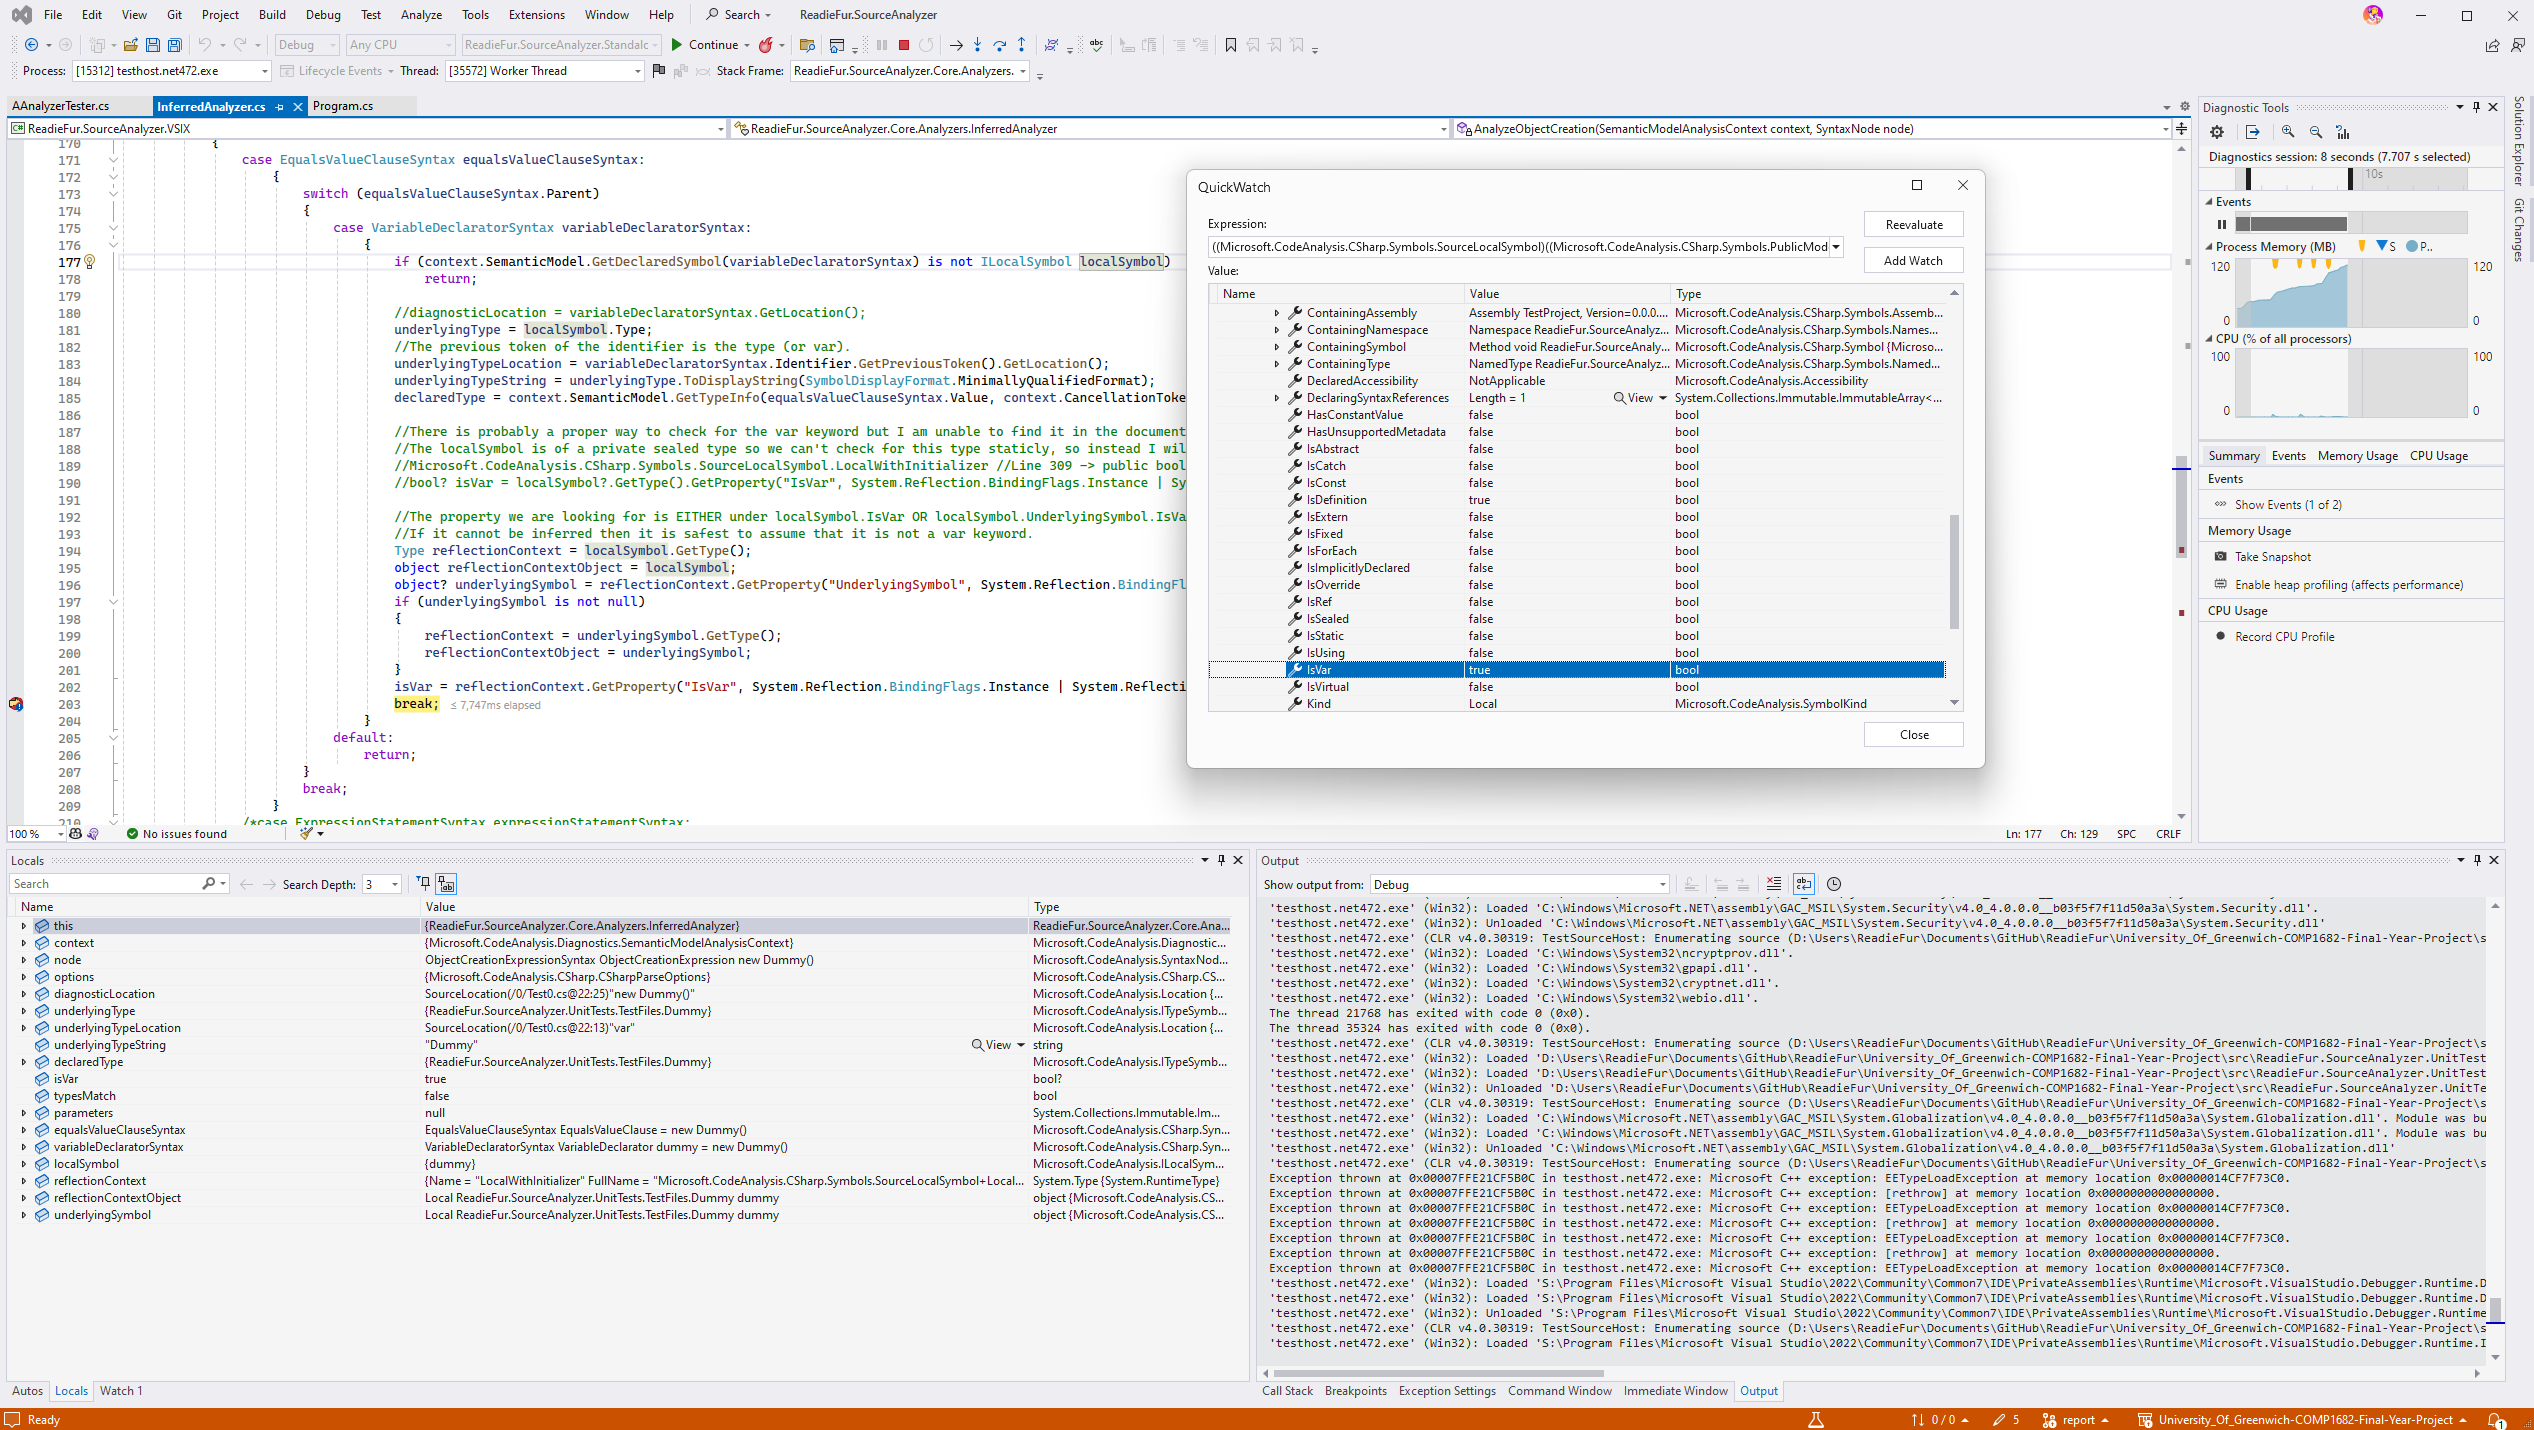
\includegraphics[width=1.0\textwidth]{Figures/DebuggingResearchProcess.png}
\end{figure}
